
\documentclass{article}

\usepackage[margin=1in]{geometry}
\linespread{1.2}

\usepackage{amsfonts, amsmath, authblk, graphicx, natbib}

% This nastiness for the bibliography to work both locally and on Overleaf
% https://tex.stackexchange.com/questions/623701/path-for-bib-file-working-simultaneously-in-texstudio-and-overleaf
\bibliographystyle{\ifnum\pdfstrcmp{\jobname}{output}=0 reports/apa-good\else ../apa-good\fi}

\title{Swinging, Fast and Slow:\\Interpreting variation in baseball swing tracking metrics}
\author[1]{Scott Powers}
\author[2]{Ronald Yurko}
\affil[1]{Department of Sport Management, Rice University}
\affil[2]{Department of Statistics \& Data Science, Carnegie Mellon University}

\begin{document}

  \maketitle
	
  \begin{abstract}
    The abstract goes here.
  \end{abstract}

  \section{Introduction}
  \label{sec:introduction}

    \begin{figure}
      \centering
      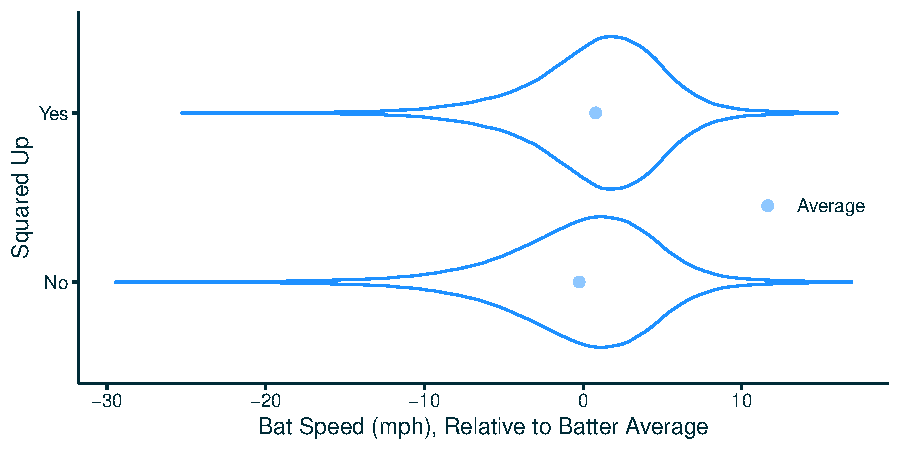
\includegraphics[width = 0.8\textwidth]{../../figures/counterintuitive.pdf}
      \caption{\it Distribution of bat speed relative to batter average by contact quality (squared up or not), across all swings in the dataset. The x-axis represents the difference between the bat speed and the batter's average bat speed. Following MLB's definition, a swing is considered ``squared up'' if the batted ball's exit velocity is at least 80\% of the theoretical maximum (given pitch speed and bat speed), a proxy for good contact.}
      \label{fig:counterintuitive}
    \end{figure}

    \begin{figure}
      \centering
      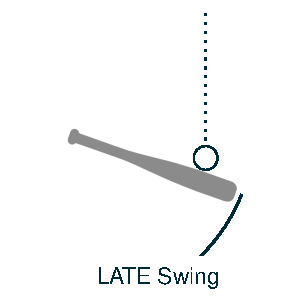
\includegraphics[width = 0.4\textwidth]{../../figures/swing_late.pdf}
      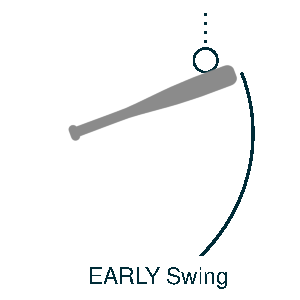
\includegraphics[width = 0.4\textwidth]{../../figures/swing_early.pdf}
      \caption{\it A diagram illustrating the effect of swing timing on swing length measurement due to the fact that swing length is measured at the point of contact. Imagining two swings with the exact same mechanics, the left image shows the swing length measurement if the swing is late, and the right image shows the swing length measurement if the swing is early.}
      \label{fig:swing-diagram}
    \end{figure}

    \subsection{Related Work}
    \label{sec:related-work}

  \section{Data}
  \label{sec:data}

  \section{Methods}
  \label{sec:methods}

    \subsection{Intention Model}
    \label{sec:methods-intention}

    We begin with the hypothesis that two covariates explain real (non-artifactual) differences in swing mechanics: ball-strike count and pitch location. To the extent that a batter’s swing tracking metrics co-vary with count, we describe this as their \textit{approach}. To the extent that a batter’s swing tracking metrics co-vary with pitch location, we describe this as swing \textit{adaptation}. Acknowledging that swing timing biases the measurement of bat speed and swing length, we mitigate this confounding bias by filtering on swings that result in squared-up contact against pitchers' primary fastballs. Additionally, based on visualizations of batter swing length and bat speed distributions (such as examples in INSERT FIGURE REFERENCE?) we are also interested in capturing variation in the shape of the intended distributions for hitters. 

    To this end, we fit the following skew-normal (SK) multilevel model:

    \begin{align}
    \begin{split}
        ( \mbox{swing length} )_i &\sim \mbox{SK}(\mu_i, \sigma, \alpha_i) \\
        \mu_i &= \mu_0 + \gamma_{p_i} + \gamma_{b_i}
        + \beta^B \cdot (\mbox{balls})_i
          + (\beta^S + \gamma^S_{b_i}) \cdot (\mbox{strikes})_i\\
        & + (\beta^X + \gamma^X_{b_i}) \cdot (\mbox{pitch loc x})_i
          + (\beta^Z + \gamma^Z_{b_i}) \cdot (\mbox{pitch loc z})_i \\
          \alpha_i &= \alpha_0 + \nu_{b_i}
    \end{split}
    \end{align}
    where $b_i$ denotes the batter on swing $i$ against pitcher $p_i$. We use the same specification for both swing length and bat speed intention models. 
    
    In detail, the $\gamma$ parameters are random intercepts and random slopes describing the mean of the swing distribution such that,

    \begin{align}
        \begin{split}
            \gamma_{p_i} &\sim \mathcal{N}(0, \tau^2_p) \\
            \boldsymbol{\gamma}_{b_i} &\sim \mathcal{N}(\boldsymbol{0}, \Sigma)
        \end{split}
    \end{align}
    where $\boldsymbol{\gamma}_{b_i}$ is the vector of batter random intercept and slopes $(\gamma_{b_i}, \gamma^S_{b_i}, \gamma^X_{b_i}, \gamma^Z_{b_i})$ which follow a multivariate normal distribution centered around the zero vector $\boldsymbol{0}$ with covariance matrix $\Sigma$. This allows us to quantify variation between hitters and pitchers at the intercept level, as well as capture variation in batter approach and swing adaptation.
    
    The $\nu_{b_i}$ parameters are random intercepts enabling us to capture variation between batters in the shape $\alpha$ of the swing length and bat speed distributions, where
    \begin{equation}
        \nu_{b_i} \sim \mathcal{N}(0, \sigma^2_p).
    \end{equation}

    These models tell us: What are the bat speed and swing length (by batter, count and pitch location) when the timing is good? We interpret the prediction from this model on each pitch as the intended bat speed and swing length.
    
    We fit both bat speed and swing length models in a Bayesian framework via the brms package in R \citep{brms}, which provides an interface for Bayesian modeling with Stan \citep{carpenter2017stan}. We use weakly informative priors for the parameters, with vague half-$t_3$ priors (i.e., a Student's $t$ distribution centered at zero with 3 degrees of freedom but truncated to positive values) for the standard deviation parameters \citep{gelman2006prior} and the LKJ prior for the correlations between batter-level effects \cite{lewandowski2009generating}. Our Bayesian approach naturally provides uncertainty quantification for the model parameters via their posterior distributions, which are estimated using MCMC sampling. For model fitting, we use four parallel chains, each with 4,000 iterations and 2,000 burn-in samples. We observe good evidence of convergence of the MCMC algorithm with trace plots and observing $\hat{R}$ statistics being close to 1 \citep{gelman1992inference, brooks1998general}, along with no indication of problematic effective sample sizes \citep{gelman2020bayesian}. 
    
    For comparison, we also fit we evaluated the skew Normal fit with simpler Gaussian fit that does not include varying intercepts controlling the skewness of the intended swing length and bat speed distributions. We use an 80/20 split to evaluate the two approaches out-of-sample. We compute the ELPD [INSERT CITATION] and ultimately observe that the skew Normal is a better fit for both bat speed and swing length. (Maybe put this conclusion in the results?)




    \subsection{Causal Model}
    \label{sec:methods-causal}

    \subsection{Run Value Model}
    \label{sec:methods-value}

  \section{Results}
  \label{sec:results}

    \subsection{Intention Model}
    \label{sec:results-intention}

      \begin{figure}
        \centering
        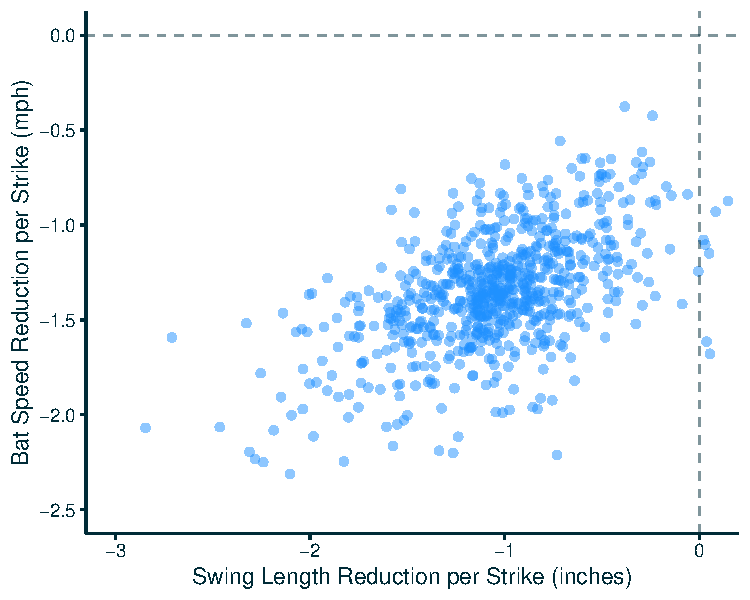
\includegraphics[width = 0.6\textwidth]{../../figures/approach.pdf}
        \caption{\it Estimated batter random slopes for strikes in the intention model. Each point is a batter $b$, with the x-value representing $\hat\beta^S + \hat\gamma^S_b$ from the model (\ref{eqn:intention-swing-length}) and the y-value representing the same quantity from the model (\ref{eqn:intention-bat-speed}). This quantity is interpretable as the expected change in swing length (or bat speed) corresponding to a one-strike increase in the ball-strike count.}
        \label{fig:approach}
      \end{figure}

    \subsection{Causal Model}
    \label{sec:results-causal}

      The previous section demonstrates that there are differences between batters in how they modulate their swing length and bat speed as the number of strikes in the count increases. This section addresses the consequences of those differences between batters. As described in Section \ref{sec:methods-causal}, we estimate three separate regression models with instrumental variables for contact probability given swing (\ref{eqn:causal-model-contact}), fair ball probability given contact (\ref{eqn:causal-model-fair}) and expected xwOBAcon given fair ball (\ref{eqn:causal-model-hit}). The estimated effects of bat speed appraoch and swing length approach from these models are reported in Table \ref{tab:causal-model}.

      \begin{table}
        \centering
        \begin{tabular}{l|r|r|r|}
          & Contact Model (\ref{eqn:causal-contact}) & Fair/Foul Model (\ref{eqn:causal-fair}) & xwOBAcon Model (\ref{eqn:causal-hit})\\
          \hline
          \begin{tabular}{l|r|r|r|}
    & Contact Model (\ref{eqn:causal-contact}) & Fair/Foul Model (\ref{eqn:causal-fair}) & xLW Model (\ref{eqn:causal-hit})\\
  \hline
  Bat Speed Approach (mph) & $-0.177 \pm0.016$ & $-0.075 \pm0.014$ & $0.023 \pm0.004$ \\ 
  Swing Length Approach (inches) & $-0.050 \pm0.010$ & $0.003 \pm0.009$ & $0.000 \pm0.002$ 
\end{tabular}
        \end{tabular}
        \caption{\it Estimated regression coefficients and corresponding standard errors from the causal models (\ref{eqn:causal-contact})--(\ref{eqn:causal-hit}). Bat Speed Approach is defined as the batter's change in bat speed per strike added to the count, as estimated by (\ref{eqn:intention-bat-speed}). Swing Length Approach is defined analogously as the batter's change in swing length per strike added to the count, as estimated by (\ref{eqn:intention-swing-length}).}
        \label{tab:causal-model}
      \end{table}

      From the contact model, the negative coefficient $-0.177$ for bat speed approach shows that batters who reduce their bat speed more per strike (i.e. more negative bat speed approach) make contact more often in 1-strike and 2-strike counts. Similarly, the negative coefficient for swing length approach shows that batters who reduce their swing length more per strike make contact more often in these counts. These results match our intuition from baseball domain knowledge: More conservative swings are more likely to make contact, a more plausible conclusion than the counterintuitive results from the naive analysis shown in Figure \ref{fig:counterintuitive}. Bat speed approach and swing length approach have similar between-batter variance, so in comparing the coefficients we observed that bat speed approach has a much greater effect (more than 3x) on contact than does swing length approach. The fair ball probability model shows a similar effect direction for bat speed approach and no effect for swing length approach.

      From the xwOBAcon model (i.e. the ``power'' model), the positive coefficient $0.023$ for bat speed approach shows that batters who reduce their bat speed more per strike (i.e. more negative bat speed approach) exhibit less power in 1-strike and 2-strike counts when they do make contact. This demonstrates evidence for the intuitive tradeoff involved when taking more conservative swings when facing more strikes: greater contact but less power. Swing length approach does not seem to have an effect on power.

      \begin{figure}
        \centering
        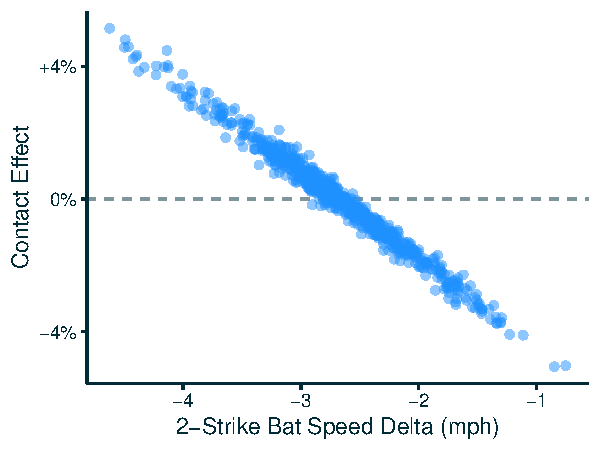
\includegraphics[width = 0.49\textwidth]{../../figures/bat_speed_contact.pdf}
        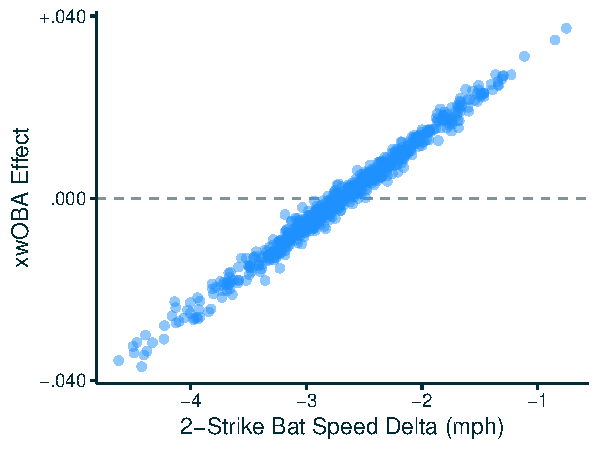
\includegraphics[width = 0.49\textwidth]{../../figures/bat_speed_power.pdf}
        \caption{\it Estimated causal effect of bat speed on contact (left) and power (right). Each point is a batter; the x-axis shows how much the batter slows their swing in two-strike counts, relative to zero-strike counts, from the model (\ref{eqn:intention-bat-speed}); the y-axis shows the estimated combined effect of the batter's bat speed and swing length adjustments on contact rate (left) and xwOBAcon (right) in two-strike counts, from the model (\ref{eqn:causal}). Contact rate is the percentage of swings contacting the ball, and xwOBAcon is a standard sabermetric statistic for measuring power. Its units are runs per plate appearance.}
        \label{fig:results-causal}
      \end{figure}

      The magnitudes of the coefficients in Table \ref{tab:causal-model} are difficult to interpret because two of the models are logistic regressions, so the coefficients represent additive effects in the log-odds scale. For example, a pitch with almost 0\% contact probability will still have almost 0\% contact probability, regardless of approach. The effect of approach on contact is maximized for pitches near 50\% contact probability. Figure \ref{fig:approach} conveys the average effect size across all 2-strike pitches. We observe that the approach effects for almost all batters (relative to an average approach) are within $\pm4\%$ contact probability and $\pm.040$ xwOBA, i.e. $\pm 40$ points of xwOBA.

    \subsection{Run Value Model}
    \label{sec:results-value}

      The previous section demonstrates that there is a contact/power tradeoff involved when batters modulate their swing length and bat speed as the number of strikes in the count increases. This section addresses whether the tradeoff is worthwhile. As described in Section \ref{sec:methods-value}, we estimate the expected linear weight of plate appearance outcomes for the average batter if they were to adopt different approaches. Figure \ref{fig:approach-run-value} plots batter approaches (as previously plotted in Figure \ref{fig:approach}) now with a color gradient in the background showing the estimated run value of each approach.

      \begin{figure}
        \centering
        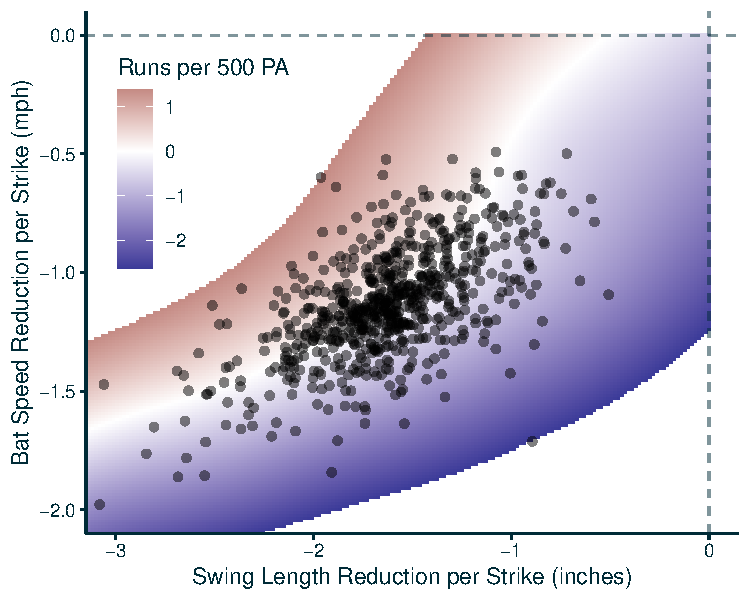
\includegraphics[width = 0.8\textwidth]{../../figures/approach_run_value.pdf}
        \caption{\it Estimated causal effect of batters' approaches, measured on the scale of runs per 500 plate appearances (PA). This figure shows the same data as Figure \ref{fig:approach} except that the background gradient reports the estimated run value of each approach. If an approach is valued at z runs, the interpretation is that the average batter with this approach is expected to produce z runs more than if they adopted an average approach, as measured by linear weights.}
        \label{fig:approach-run-value}
      \end{figure}

      The magnitude of the difference between the higest-value approaches and the lowest-value approaches is small, approximately 4 runs per 500 plate appearances. To put this in context, it amounts to a difference of roughly half a win per season[CITATION]. Baseball teams are chasing increasingly small competitive advantages[CITATION], and the cost of half a win is roughly \$5 million in the free agent market[CITATION]. We observe that the highest-value approaches are those which cut down on swing length without cutting down on bat speed. From Table \ref{tab:causal-model}, we can see that this is a way to avoid the contact/power tradeoff because cutting down on swing length (all else equal) increases contact without decreasing power.

      \begin{table}
        \centering
        \begin{tabular}{rl|rr|r}
          &        & \multicolumn{2}{c|}{Approach}          & Runs /\\
          & Batter & Bat Speed (mph)  & Swing Length (in.)  & 500 PA\\
          \hline
          \begin{tabular}{rl|rr|r}
& & \multicolumn{2}{c|}{Approach} & Runs /\\
 & Batter & Bat Speed (mph) & Swing Length (in.) & 500 PA \\
% latex table generated in R 4.5.0 by xtable 1.8-4 package
% Tue Jul  1 14:15:51 2025
  \hline
  1 & Matt Chapman & $-0.60$ & $-1.96$ & $1.39$ \\ 
    2 & Matt Olson & $-0.64$ & $-1.88$ & $1.21$ \\ 
    3 & Mark Canha & $-1.14$ & $-2.51$ & $1.13$ \\ 
    4 & Dominic Fletcher & $-1.07$ & $-2.36$ & $1.12$ \\ 
    5 & Joey Bart & $-0.83$ & $-1.95$ & $1.04$ \\ 
   &  &  &  &  \\ 
  688 & Jeimer Candelario & $-1.71$ & $-1.88$ & $-1.52$ \\ 
  689 & Chas McCormick & $-1.42$ & $-1.00$ & $-1.60$ \\ 
  690 & Trea Turner & $-1.64$ & $-1.54$ & $-1.62$ \\ 
  691 & Jake McCarthy & $-1.84$ & $-1.91$ & $-2.02$ \\ 
  692 & Santiago Espinal & $-1.71$ & $-0.89$ & $-2.65$ \\ 
\end{tabular}

        \end{tabular}
        \caption{\it Top 5 and bottom 5 approaches, ranked by runs per 500 plate appearances (PA). Bat Speed Approach and Swing Length Approach are the batter's change in bat speed and swing length, respectively, per strike added to the count. We estimate the effect that each approach would have on the average batter's performance, as measured on the run scale via linear weights.}
        \label{tab:approach-ranked}
      \end{table}

      Table \ref{tab:approach-ranked} reports the specific approaches and corresponding run values of the top 5 and bottom 5 batters, ranked according to the run value of their approaches {\it applied to an average batter}. Interestingly, three of the top four batters (Chapman, Olson and Canha) all spent the first five or more seasons of their MLB careers with the Oakland Athletics. At the other end of the table, Rizzo and Turner are very highly accomplished batters. The spread of overall batter talent is much greater than the small spread explained by approach.

    \subsection{Other Sources of Swing Variation}
    \label{sec:results-other}

      \begin{figure}
        \centering
        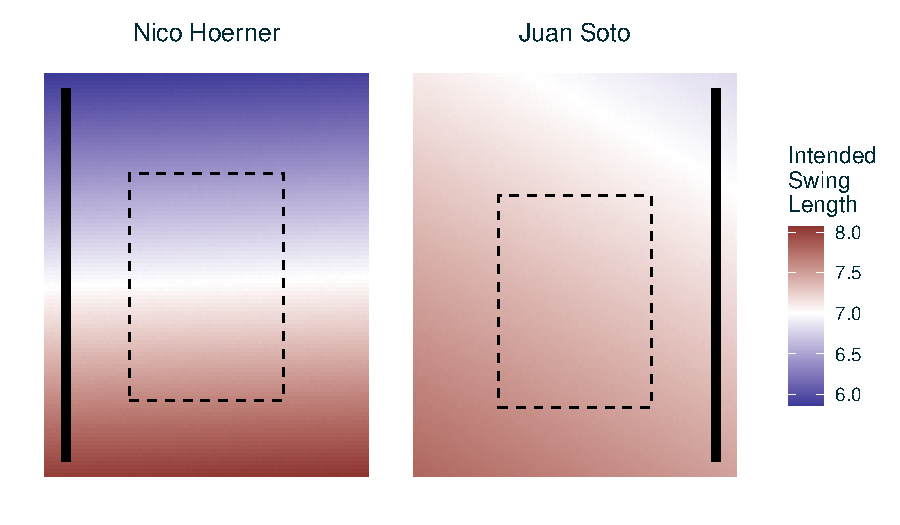
\includegraphics[width = 0.8\textwidth]{../../figures/adaptation.pdf}
        \caption{\it Expected swing length by pitch location for two sample batters: Nico Hoerner (left) and Juan Soto (right), from the perspective of behind home plate. The thick vertical bars show the side of the plate on which the batter stands, and the dashed rectangle shows the strike zone, which depends on the height and stance of the batter. The color shows the predicted swing length  from model (\ref{eqn:intention-swing-length}) assuming a 0-0 count.}
        \label{fig:adaptation}
      \end{figure}

  \section{Discussion}
  \label{sec:discussion}

    \subsection{Future Work}
    \label{sec:future-work}

      \begin{itemize}
        \item batter-specific approach values (as opposed to applying approach to average batter)
        \item valuing tradeoffs considering base-out situation (e.g. runner on third, less than two outs)
        \item future data coming down the pipeline from MLBAM
      \end{itemize}

  % This nastiness for the bibliography to work both locally and on Overleaf
  % https://tex.stackexchange.com/questions/623701/path-for-bib-file-working-simultaneously-in-texstudio-and-overleaf
  \bibliography{\ifnum\pdfstrcmp{\jobname}{output}=0 reports/swingfastslow\else ../swingfastslow\fi}

\end{document}